
Um Hinweise auf einen möglichen Zusammenhang der Treppengeschwindigkeit mit weiteren durch das Messexperiment ermittelten Größen zu finden, wird eine lineare 
Regression angewandt.

Die hier betrachteten Größen sind Wunschgeschwindigkeit (in der Ebene),
Körpergröße und Rundennummer. Es wird gesondert die Treppengeschwindigkeit aufwärts und abwärts betrachtet.
Zunächst wird nur auf eine Abhängigkeit überprüft, danach die Abhängigkeit von mehreren kombinierten Größen. Die Zusammenhänge werden bezüglich ihrer Plausibilität bewertet.

\subsection{Prüfung auf eine einfache Abhängigkeit}

Hier werden sechs Gleichungen mittels linearer Regression ermittelt: 

\[v_{auf}(v_{ebene}) = \beta_0 + \beta_1 v_{ebene}\]
\[v_{ab}(v_{ebene}) = \beta_0 + \beta_1 v_{ebene}\]

\[v_{auf}(groesse) = \beta_0 + \beta_1 groesse\]
\[v_{ab}(groesse) = \beta_0 + \beta_1 groesse\]

\[v_{auf}(runde) = \beta_0 + \beta_1 runde\]
\[v_{ab}(runde) = \beta_0 + \beta_1 runde\]

\subsubsection{Wunschgeschwindigkeit in der Ebene}

Für die Abhängigkeit Wunschgeschwindigkeit in der Ebene wurde 
der Zusammenhang wie in den Formeln für die Treppengeschwindigkeit aufwärts (\ref{eq:auf2017-ebene}) und abwärts (\ref{eq:ab2017-ebene}) ermittelt. 

\begin{equation} \label{eq:auf2017-ebene}
	v_{auf}(v_{ebene}) = 0.294389 + 0.393467 v_{ebene}
\end{equation}
\begin{equation} \label{eq:ab2017-ebene}
	v_{ab}(v_{ebene}) = 0.475883 + 0.453419 v_{ebene}
\end{equation}

Beide Steigungen sind positiv. Hat ein Proband eine schnellere Wunschgeschwindigkeit in der Ebene, verhält er sich auch schneller auf 
der Treppe. Die Abbildungen \ref{fig:auf2017-ebene} und \ref{fig:ab2017-ebene}
stellen dies grafisch dar. 

\begin{figure} \centering 
	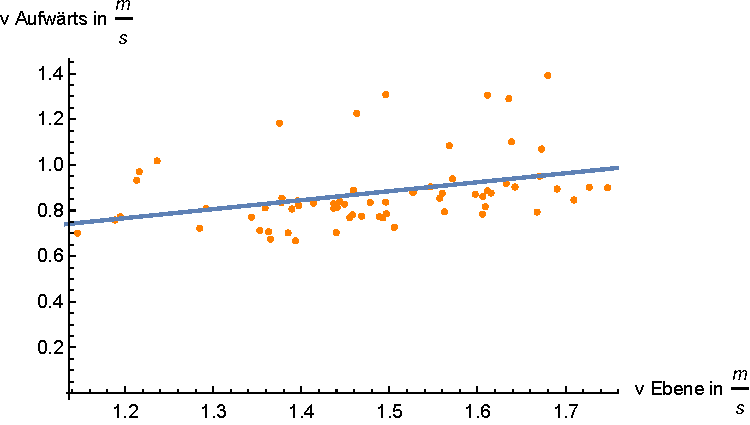
\includegraphics[]{abbildungen/regression/2017/auf-ebene.pdf}
	\[\begin{array}{l|llll}
 \text{} & \text{Estimate} & \text{Standard Error} & \text{t-Statistic} & \text{P-Value} \\
\hline
 1 & 0.506746 & 0.0900029 & 5.63033 & \text{2.603647901106944$\grave{ }$*${}^{\wedge}$-6} \\
 \text{vEbene} & 0.168071 & 0.0588553 & 2.85567 & 0.00727064 \\
\end{array}\]


	\caption{Abhängigkeit Wunschgeschwindigkeit in der Ebene zur Treppengeschwindigkeit aufwärts. Messdaten (orange) mit ermittelter Regressionsgerade (blau). \label{fig:auf2017-ebene}}
\end{figure}

\begin{figure} \centering 
	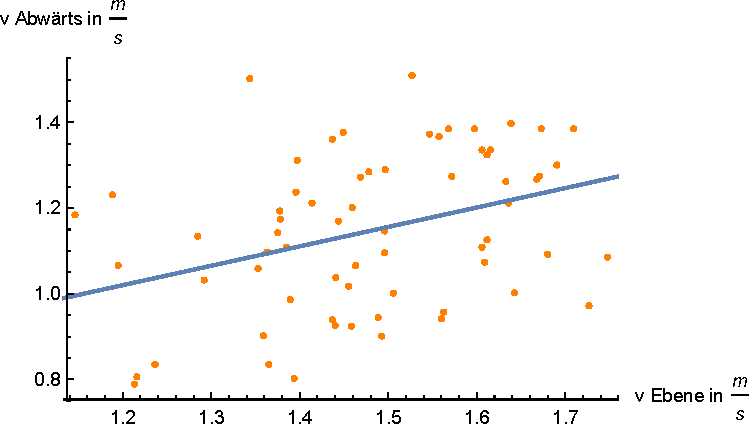
\includegraphics[]{abbildungen/regression/2017/ab-ebene.pdf}
	\[\begin{array}{l|llll}
 \text{} & \text{Estimate} & \text{Standard Error} & \text{t-Statistic} & \text{P-Value} \\
\hline
 1 & 0.440848 & 0.213068 & 2.06904 & 0.0428577 \\
 \text{vEbene} & 0.478525 & 0.142985 & 3.34668 & 0.00141579 \\
\end{array}\]


	\caption{Abhängigkeit Wunschgeschwindigkeit in der Ebene zur Treppengeschwindigkeit abwärts. Messdaten (orange) mit ermittelter Regressionsgerade (blau). \label{fig:ab2017-ebene}}
\end{figure}

In Abbildung \ref{fig:auf2017-ebene} sind wieder
deutlich die schon in der Betrachtung zur Normalverteilung erwähnten Ausreißer zu erkennen. Deshalb wurde die lineare Regression für den gefilterten Messdatensatz (nur Datensätze ohne Bemerkung) durchgeführt. Es ergeben sich neue Formeln für die Treppengeschwindigkeit aufwärts (\ref{eq:ohne-auf2017-ebene}) und abwärts (\ref{eq:ohne-ab2017-ebene}). Dazu gehören Abbildungen \ref{fig:ohne-auf2017-ebene} und \ref{fig:ohne-ab2017-ebene}. Die Ausreißer wurden in der Regression hier nicht verwendet, sind aber hervorgehoben eingezeichnet. Bei der Treppengeschwindigkeit aufwärts sind es deutlich mehr Ausreißer und sie fallen alle in den schnelleren Bereich. Die Regressionsgerade für die Daten ohne Ausreißer liegt dementsprechend 
etwas weiter unter (langsamer) im Vergleich zu Abbildung \ref{fig:auf2017-ebene}. Bei Abbildung \ref{fig:ohne-ab2017-ebene} sind es nur 
vier Ausreißer. Sie sind auch stärker gestreut. Die Regressionsgerade für den Zusammenhang zur Geschwindigkeit abwärts wird nicht besonders von dem Weglassen der Ausreißer beeinflusst. Die Ausreißer werden in den weiteren Regressionen nicht genauer betrachtet. Alle Abbildungen und Plausibilisierungstests dazu sind aber als Dateien angelegt.

\begin{equation} \label{eq:ohne-auf2017-ebene}
	v'_{auf}(v_{ebene}) = 0.332577 + 0.325892 v_{ebene}
\end{equation}
\begin{equation} \label{eq:ohne-ab2017-ebene}
	v'_{ab}(v_{ebene}) = 0.440848 + 0.478525 v_{ebene}
\end{equation}

\begin{figure} \centering 
	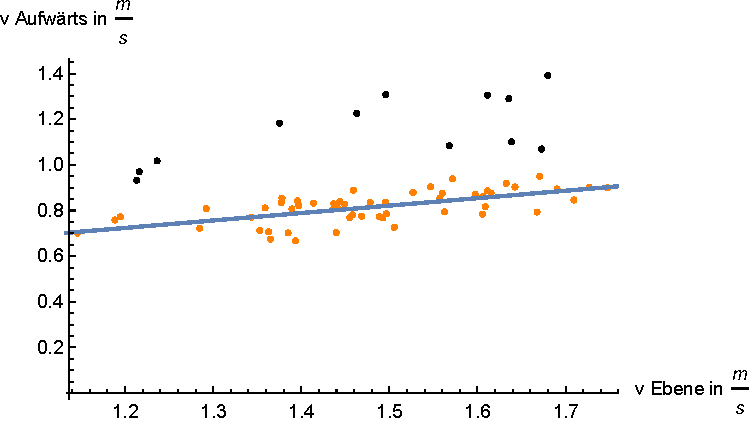
\includegraphics[]{abbildungen/regression/2017/ohneausreisser/auf-ebene.pdf}
	\[\begin{array}{l|llll}
 \text{} & \text{Estimate} & \text{Standard Error} & \text{t-Statistic} & \text{P-Value} \\
\hline
 1 & 0.506746 & 0.0900029 & 5.63033 & \text{2.603647901106944$\grave{ }$*${}^{\wedge}$-6} \\
 \text{vEbene} & 0.168071 & 0.0588553 & 2.85567 & 0.00727064 \\
\end{array}\]


	\caption{Abhängigkeit Wunschgeschwindigkeit in der Ebene zur Treppengeschwindigkeit aufwärts. Gefilterte Messdaten (orange) und Ausreißer (schwarz) mit ermittelter Regressionsgerade (blau). \label{fig:ohne-auf2017-ebene}}
\end{figure}

\begin{figure} \centering 
	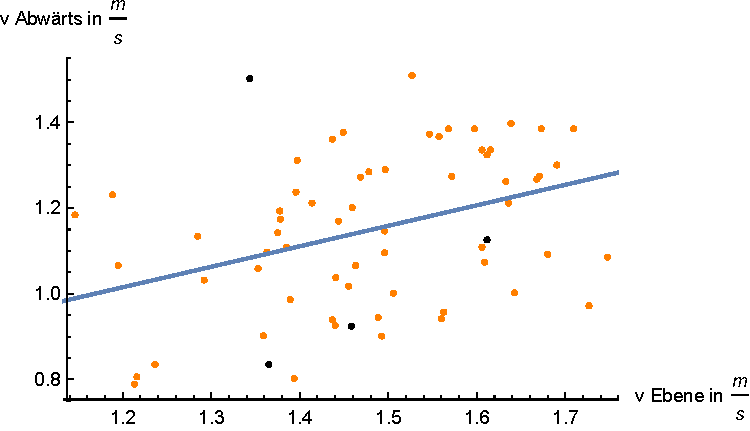
\includegraphics[]{abbildungen/regression/2017/ohneausreisser/ab-ebene.pdf}
	\[\begin{array}{l|llll}
 \text{} & \text{Estimate} & \text{Standard Error} & \text{t-Statistic} & \text{P-Value} \\
\hline
 1 & 0.440848 & 0.213068 & 2.06904 & 0.0428577 \\
 \text{vEbene} & 0.478525 & 0.142985 & 3.34668 & 0.00141579 \\
\end{array}\]


	\caption{Abhängigkeit Wunschgeschwindigkeit in der Ebene zur Treppengeschwindigkeit abwärts. Gefilterte Messdaten (orange) und Ausreißer (schwarz) mit ermittelter Regressionsgerade (blau).
	\label{fig:ohne-ab2017-ebene}}
\end{figure}

Für die Plausibilisierung der Regression wird die Nullhypothese 
$H_0: \beta_1 = 0$ aufgestellt. Signifikanzniveau $\alpha = 0.05$.
Die Ergebnisse des Tests sind in Abbildung \ref{fig:auf2017-ebene} zu sehen.
Signifikanz liegt vor, weil $p < \alpha$. Man verwirft die
Nullhypothese. Kein Einfluss von $v_{ebene}$ auf $v_{auf}$ wäre unplausibel, wenn auch nicht ausgeschlossen.

Die Nullhypothese und das Signifikanzniveau sind für alle folgenden Regressionen gleich. Die Ergebnisse für den Abstieg sind in Abbildung \ref{fig:ab2017-ebene} zu sehen.
Signifikanz liegt vor, weil $p < \alpha$. Man verwirft die
Nullhypothese. Kein Einfluss von $v_{ebene}$ auf $v_{ab}$ wäre unplausibel, wenn auch nicht ausgeschlossen.

\subsubsection{Körpergröße}

Für die Abhängigkeit Körpergröße wurde 
der Zusammenhang (\ref{eq:auf2017-groesse}) und (\ref{eq:ab2017-groesse}) ermittelt.

\begin{equation} \label{eq:auf2017-groesse}
	v_{auf}(groesse) = 0.133389 + 0.00419914 groesse
\end{equation}
\begin{equation} \label{eq:ab2017-groesse}
	v_{ab}(groesse) = 1.59558 - 0.00253145 groesse
\end{equation}

In den Abbildungen \ref{fig:auf2017-groesse} und \ref{fig:ab2017-groesse} ist 
zu sehen, dass nach dem Modell größere Personen leicht schneller Treppen besteigen, aber beim herabsteigen etwas langsamer als kleinere
Personen sind. 

\begin{figure} \centering 
	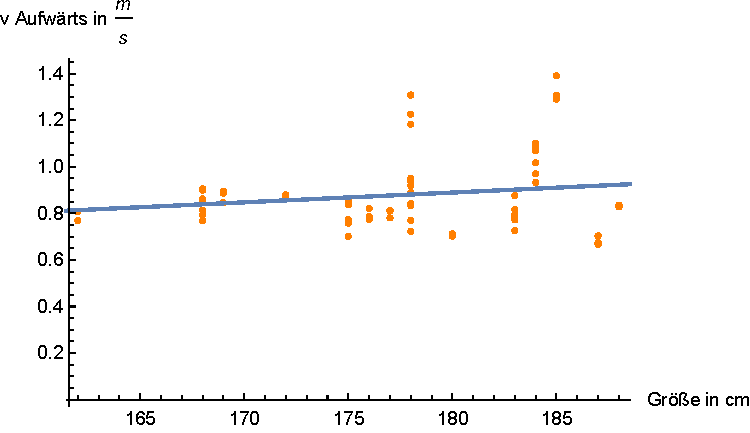
\includegraphics[]{abbildungen/regression/2017/auf-groesse.pdf}
	\[\begin{array}{l|llll}
 \text{} & \text{Estimate} & \text{Standard Error} & \text{t-Statistic} & \text{P-Value} \\
\hline
 1 & 1.42188 & 0.660147 & 2.15388 & 0.0335816 \\
 \text{gr{\" o}{\ss}e} & -0.00301832 & 0.0037105 & -0.813455 & 0.417834 \\
\end{array}\]


	\caption{Abhängigkeit Körpergröße zur Treppengeschwindigkeit aufwärts. Messdaten (orange) mit ermittelter Regressionsgerade (blau). \label{fig:auf2017-groesse}}
\end{figure}

\begin{figure} \centering 
	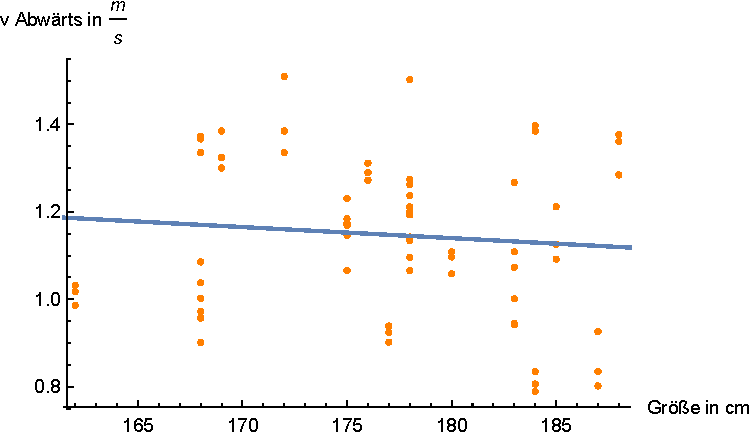
\includegraphics[]{abbildungen/regression/2017/ab-groesse.pdf}
	\[\begin{array}{l|llll}
 \text{} & \text{Estimate} & \text{Standard Error} & \text{t-Statistic} & \text{P-Value} \\
\hline
 1 & 1.59558 & 0.582855 & 2.73753 & 0.00800578 \\
 \text{gr{\" o}{\ss}e} & -0.00253145 & 0.00328881 & -0.769715 & 0.444301 \\
\end{array}\]


	\caption{Abhängigkeit Körpergröße zur Treppengeschwindigkeit abwärts. Messdaten (orange) mit ermittelter Regressionsgerade (blau). \label{fig:ab2017-groesse}}
\end{figure}

Ergebnisse der Plausibilisierung für den Aufstieg 
(Abbildung \ref{fig:auf2017-groesse}):
Signifikanz liegt nicht vor, weil $p > \alpha$. Man nimmt die
Nullhypothese an. Kein Einfluss von $groesse$ auf $v_{auf}$ ist plausibel.

Ergebnisse der Plausibilisierung für den Abstieg
(Abbildung \ref{fig:ab2017-groesse}):
Signifikanz liegt vor, weil $p > \alpha$. Man nimmt die
Nullhypothese an. Kein Einfluss von $groesse$ auf $v_{ab}$ ist plausibel.


\subsubsection{Rundennummer}


Für die Abhängigkeit Rundennummer wurde 
der Zusammenhang (\ref{eq:auf2017-runde}) und (\ref{eq:ab2017-runde}) ermittelt.

\begin{equation} \label{eq:auf2017-runde}
v_{auf}(runde) = 0.890435 - 0.00670795 runde
\end{equation}
\begin{equation} \label{eq:ab2017-runde}
v_{ab}(runde) = 1.14614\, +0.000574582 runde
\end{equation}

In den Abbildungen \ref{fig:auf2017-runde} und \ref{fig:ab2017-runde} ist 
zu sehen, dass sich nach dem Modell die Treppengeschwindigkeit bei Änderung der Runde fast nicht ändert. 

\begin{figure} \centering 
	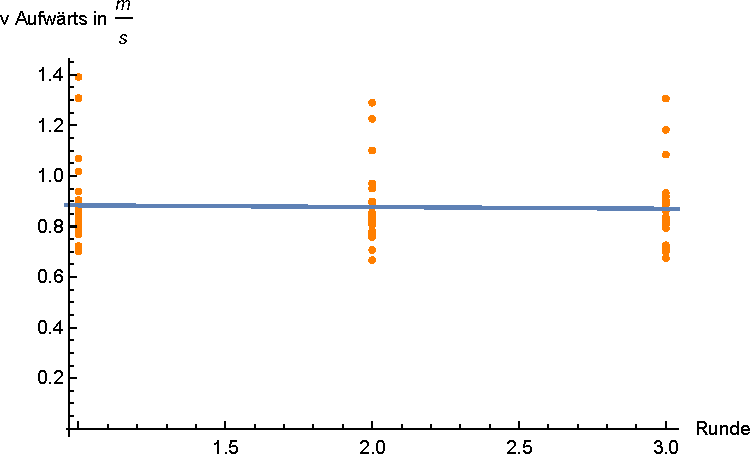
\includegraphics[]{abbildungen/regression/2017/auf-runde.pdf}
	\[\begin{array}{l|llll}
 \text{} & \text{Estimate} & \text{Standard Error} & \text{t-Statistic} & \text{P-Value} \\
\hline
 1 & 0.94804 & 0.2081 & 4.55569 & 0.0000551454 \\
 \text{runde} & -0.0241206 & 0.0963317 & -0.250391 & 0.80367 \\
\end{array}\]


	\caption{Abhängigkeit Rundennummer zur Treppengeschwindigkeit aufwärts. Messdaten (orange) mit ermittelter Regressionsgerade (blau). \label{fig:auf2017-runde}}
\end{figure}

\begin{figure} \centering 
	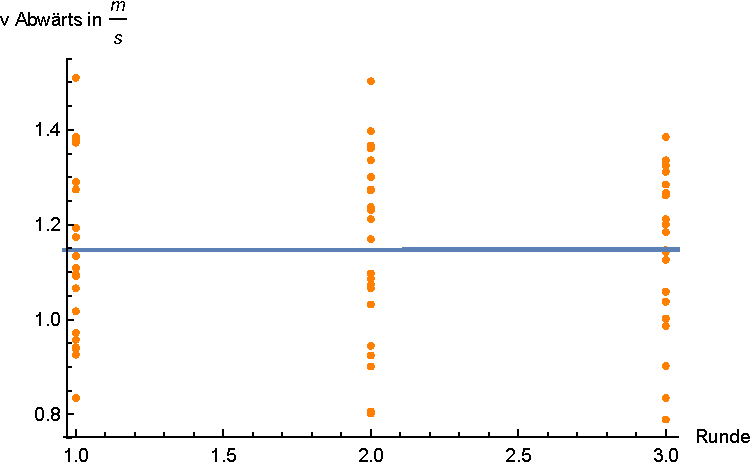
\includegraphics[]{abbildungen/regression/2017/ab-runde.pdf}
	\[\begin{array}{l|llll}
 \text{} & \text{Estimate} & \text{Standard Error} & \text{t-Statistic} & \text{P-Value} \\
\hline
 1 & 0.859522 & 0.0289618 & 29.6777 & \text{6.817362585804904$\grave{ }$*${}^{\wedge}$-26} \\
 \text{runde} & 0.00475595 & 0.0134067 & 0.354744 & 0.724973 \\
\end{array}\]


	\caption{Abhängigkeit Rundennummer zur Treppengeschwindigkeit abwärts. Messdaten (orange) mit ermittelter Regressionsgerade (blau). \label{fig:ab2017-runde}}
\end{figure}

Ergebnisse der Plausibilisierung für den Aufstieg
(Abbildung \ref{fig:auf2017-runde}):
Signifikanz liegt nicht vor, weil $p > \alpha$. Man nimmt die
Nullhypothese an. Kein Einfluss von $runde$ auf $v_{auf}$ ist plausibel.

Ergebnisse der Plausibilisierung für den Abstieg
(Abbildung \ref{fig:ab2017-runde}):
Signifikanz liegt vor, weil $p > \alpha$. Man nimmt die
Nullhypothese an. Kein Einfluss von $runde$ auf $v_{ab}$ ist plausibel.

\subsection{Mehrere Abhängigkeiten}

Hier werden weitere vier lineare Gleichungen mit mehreren Parametern ermittelt.

\[v_{auf}(v_{ebene}, groesse) = \beta_0 + \beta_1 v_{ebene} + \beta_2 groesse\]
\[v_{ab}(v_{ebene}, groesse) = \beta_0 + \beta_1 v_{ebene} + \beta_2 groesse\]

\[v_{auf}(v_{ebene}, groesse, runde) = \beta_0 + \beta_1 v_{ebene} + \beta_2 groesse + \beta_3 runde\]
\[v_{ab}(v_{ebene}, groesse, runde) = \beta_0 + \beta_1 v_{ebene} + \beta_2 groesse + \beta_3 runde\]

Für die Plausibilisierung der Regression wird die Nullhypothese 
$H_0: \beta_1 = 0  \lor \beta_2 = 0$ bzw. $H_0: \beta_1 = 0  \lor \beta_2 = 0 \lor \beta_3 = 0$ aufgestellt.

\subsubsection{Ebenengeschwindigkeit und Größe}

Für die Abhängigkeiten Wunschgeschwindigkeit in der Ebene und Körpergröße wurde 
der Zusammenhang (\ref{eq:auf2017-ebene-groesse}) und (\ref{eq:ab2017-ebene-groesse}) ermittelt.

\begin{equation} \label{eq:auf2017-ebene-groesse}
	v_{auf}(v_{ebene}, groesse) = -0.691667 + 0.425116 v_{ebene} + 0.00530344 groesse
\end{equation}
\begin{equation} \label{eq:ab2017-ebene-groesse}
	v_{auf}(v_{ebene}, groesse) = 0.731523 + 0.445214 v_{ebene} + -0.00137494 groesse
\end{equation}

In den Abbildungen \ref{fig:auf2017-ebene-groesse} und \ref{fig:ab2017-ebene-groesse} ist 
zu sehen, dass ein größerer Proband mit schnellerer Ebenengeschwindigkeit auch eine schnellere Treppengeschwindigkeit aufwärts erreicht. Eine schnellere Treppengeschwindigkeit abwärts wird durch einen Proband mit schnellerer Ebenengeschwindigkeit und kleinerer Größe erreicht. Eine Änderung von $50 cm$ in der Größe wirkt sich auf das Besteigen aufwärts mit ca. $0.25 m/s$ und abwärts mit ca. $0.05 m/s$ aus.

\begin{figure} \centering 
	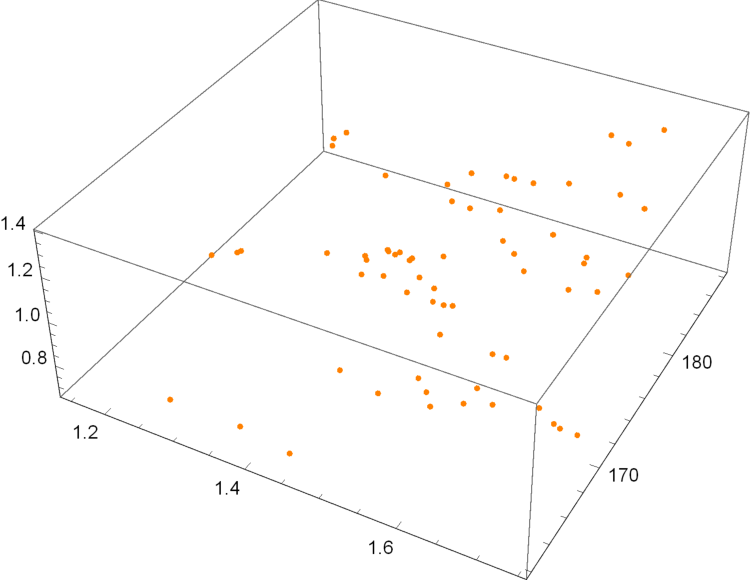
\includegraphics[]{abbildungen/regression/2017/auf-ebene-groesse.pdf}
	\[\begin{array}{l|llll}
 \text{} & \text{Estimate} & \text{Standard Error} & \text{t-Statistic} & \text{P-Value} \\
\hline
 1 & 1.0165 & 0.140132 & 7.25384 & \text{1.5820003769083974$\grave{ }$*${}^{\wedge}$-10} \\
 \text{vEbene} & 0.199894 & 0.0433176 & 4.61461 & 0.0000134806 \\
 \text{gr{\" o}{\ss}e} & -0.00294506 & 0.000643082 & -4.5796 & 0.0000154292 \\
\end{array}\]


	\caption{Abhängigkeiten Ebenengeschwindigkeit und Größe zur Treppengeschwindigkeit aufwärts. Messdaten (orange) mit ermittelter Regressionsebene (blau). \label{fig:auf2017-ebene-groesse}}
\end{figure}

\begin{figure} \centering 
	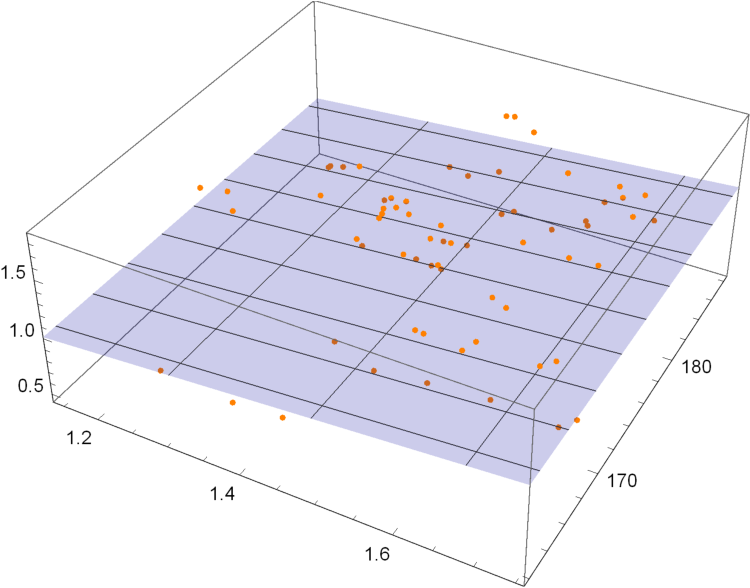
\includegraphics[]{abbildungen/regression/2017/ab-ebene-groesse.pdf}
	\[\begin{array}{l|llll}
 \text{} & \text{Estimate} & \text{Standard Error} & \text{t-Statistic} & \text{P-Value} \\
\hline
 1 & 0.701775 & 0.543236 & 1.29184 & 0.199331 \\
 \text{vEbene} & 0.696676 & 0.127843 & 5.44946 & \text{3.523565756565165$\grave{ }$*${}^{\wedge}$-7} \\
 \text{gr{\" o}{\ss}e} & -0.00382545 & 0.00268911 & -1.42257 & 0.157912 \\
\end{array}\]


	\caption{Abhängigkeiten Ebenengeschwindigkeit und Größe zur Treppengeschwindigkeit abwärts. Messdaten (orange) mit ermittelter Regressionsebene (blau). \label{fig:ab2017-ebene-groesse}}
\end{figure}

Ergebnisse der Plausibilisierung für den Aufstieg
(Abbildung \ref{fig:auf2017-ebene-groesse}):
Signifikanz liegt vor, weil beide $p < \alpha$. Man lehnt die
Nullhypothese ab. Kein Einfluss von $v_{ebene}$ und $groesse$ auf $v_{auf}$ ist unplausibel.

Ergebnisse der Plausibilisierung für den Abstieg
(Abbildung \ref{fig:ab2017-ebene-groesse}):
Signifikanz liegt nicht vor, weil $p_{\beta_2} > \alpha$. Man nimmt die
Nullhypothese an. Kein Einfluss von $v_{ebene}$ und $groesse$ auf $v_{ab}$ ist plausibel.


\subsubsection{Ebenengeschwindigkeit, Größe und Rundennummer}

Für die Abhängigkeiten Wunschgeschwindigkeit in der Ebene, Körpergröße und Rundennummer wurde 
der Zusammenhang (\ref{eq:auf2017-ebene-groesse-runde}) und (\ref{eq:ab2017-ebene-groesse-runde}) ermittelt.

\begin{multline} \label{eq:auf2017-ebene-groesse-runde}
v_{auf}(v_{ebene}, groesse, runde) = \\
-0.68569 + 0.424337 v_{ebene} + 0.00530141 groesse + -0.00223211 runde
\end{multline}
\begin{multline} \label{eq:ab2017-ebene-groesse-runde}
v_{auf}(v_{ebene}, groesse, runde) = \\
0.717358 + 0.447061 v_{ebene} + -0.00137015 groesse + 0.00529011 runde
\end{multline}

\begin{figure} \centering 
	\[\begin{array}{l|llll}
 \text{} & \text{Estimate} & \text{Standard Error} & \text{t-Statistic} & \text{P-Value} \\
\hline
 1 & 1.01208 & 0.137206 & 7.37634 & \text{2.1703587613814404$\grave{ }$*${}^{\wedge}$-8} \\
 \text{vEbene} & 0.117482 & 0.0493951 & 2.37842 & 0.0235248 \\
 \text{gr{\" o}{\ss}e} & -0.00231594 & 0.000542029 & -4.27274 & 0.000161828 \\
 \text{runde} & -0.00663057 & 0.00696761 & -0.951628 & 0.348419 \\
\end{array}\]


	\caption{Abhängigkeiten Ebenengeschwindigkeit, Größe und Runde zur Treppengeschwindigkeit aufwärts.
	\label{fig:auf2017-ebene-groesse-runde}}
\end{figure}

\begin{figure} \centering 
	\[\begin{array}{l|llll}
 \text{} & \text{Estimate} & \text{Standard Error} & \text{t-Statistic} & \text{P-Value} \\
\hline
 1 & 1.54231 & 0.231512 & 6.66191 & \text{1.6207125042011794$\grave{ }$*${}^{\wedge}$-7} \\
 \text{vEbene} & -0.070368 & 0.083346 & -0.844287 & 0.404777 \\
 \text{gr{\" o}{\ss}e} & -0.00320726 & 0.000914584 & -3.5068 & 0.00136734 \\
 \text{runde} & 0.0043198 & 0.0117567 & 0.367433 & 0.715715 \\
\end{array}\]


	\caption{Abhängigkeiten Ebenengeschwindigkeit, Größe und Runde zur Treppengeschwindigkeit abwärts.
	\label{fig:ab2017-ebene-groesse-runde}}
\end{figure}

Ergebnisse der Plausibilisierung für den Aufstieg
(Abbildung \ref{fig:auf2017-ebene-groesse-runde}):
Signifikanz liegt nicht vor, weil $p_{\beta_2} > \alpha$ und $p_{\beta_3} > \alpha$. Man nimmt die Nullhypothese an.

Ergebnisse der Plausibilisierung für den Abstieg
(Abbildung \ref{fig:ab2017-ebene-groesse-runde}):
Signifikanz liegt nicht vor, weil $p_{\beta_2} > \alpha$ und $p_{\beta_3} > \alpha$. Man nimmt die Nullhypothese an.